\subsection{I-V Method} \label{ssec:IVMethod}
The I-V method or current voltage method, has already been shortly introduced in section \ref{sec:MeasureReactiveComponents}, here it was realized by the use of a function generator and an oscilloscope. In this chapter, the I-V method will however be introduced in a more broad spectrum, that is to say, the general principle of the method will be outlined.

In general, two principles of the I-V method are implemented in the industry, either the I-V method or the RF I-V method. The I-V method offers good accuracy 
and a broad bandwidth, from a few hertz to about \SIQ{100}{\mega\hertz}. The RF I-V method uses RF principles such as directional couplers and extends the bandwidth up to about \SIQ{3}{\giga\hertz}, it is however not suitable for frequencies below the mega hertz region\cite{Keysight_Impedance}. This chapter will solely focus on the I-V method as the RF frequency range is not of interest to this project.

The principle of the I-V method is simple; measure current and voltage, and determine the angle between them. This can be implemented in numerous different ways, using coupled inductors to measure the current, or a series shunt where the voltage-drop can be measured across, to name a few. 

\begin{figure}[H]
    \centering
    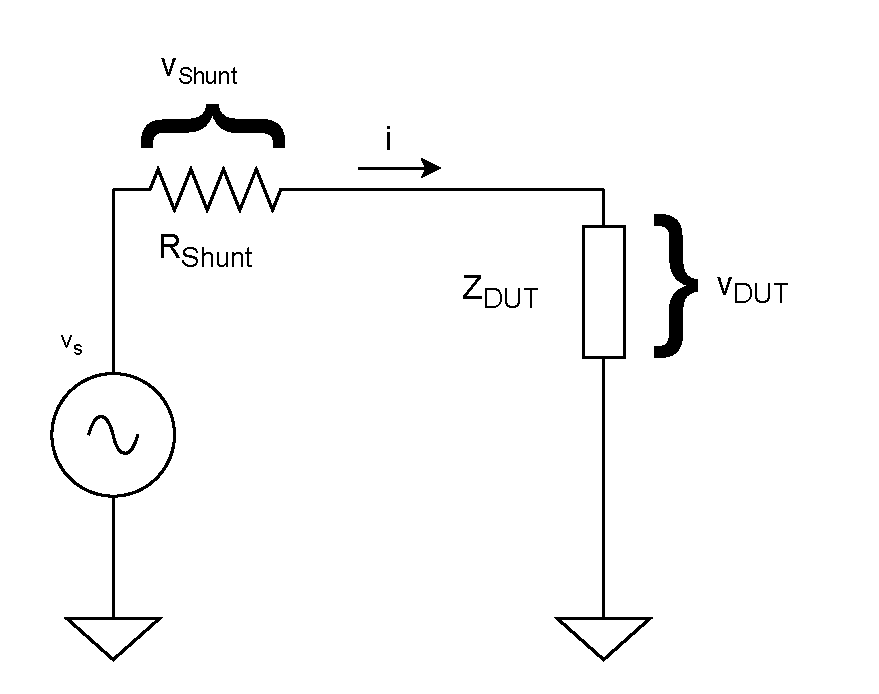
\includegraphics[width=0.75\textwidth]{Sections/4_TechnicalAnalysis/Figures_JFT/IV_Method.pdf}
    \caption{The I-V Method implemented with a current shunt to measure the current}
    \label{fig_4_2_IVMethod}
\end{figure}

The principle of the I-V method can be seen in figure \refq{fig_4_2_IVMethod}. The current in the system can be described by an amplitude and phase, as can the voltage, as seen in equation \ref{eq:4_2_2_IVVectors}, where $v$ is the voltage across the DUT and $i$ is the current through it. It is assumed that the current is the same through the shunt and the DUT.

\begin{equation}
    \label{eq:4_2_2_IVVectors}
    \begin{split}
        \bar{i} & = |i|\cdot\e ^{j\theta_i} \Rightarrow \bar{i} = \frac{|v_{shunt}|}{R_{shunt}}\e ^{j\theta_{v\:shunt}}\\
        \bar{v_{DUT}} & = |\bar{v_{DUT}}| \cdot\e ^{j\theta_{v\:DUT}}
    \end{split}
\end{equation}

The impedance can then be calculated from the two voltages of the system, i.e. the shunt voltage and the DUT voltage, as seen in equation \ref{eq:4_2_2_Impedance}.

\begin{equation}
    \label{eq:4_2_2_Impedance}
    \begin{split}
        Z & = \frac{v_{DUT}}{i} \Rightarrow \bar{Z} = \frac{|v_{DUT}| \cdot\e ^{j\theta_{v\:DUT}}}{\frac{|v_{shunt}|}{R_{shunt}}\e ^{j\theta_{v\:shunt}}} \\
        \bar{Z} & = \frac{|v_{DUT}|\cdot R_{shunt}}{|v_{shunt}|}\cdot \e ^{j\left(\theta_{v\:DUT}-\theta_{v\:shunt}\right)}
    \end{split}
\end{equation}

This is the I-V method in its simplest form. The shunt used is however required to be swapped depending on the DUT, as a small shunt would be poorly suited to measure small currents. In practice, compensation elements can also be required to ensure stability, as some systems can become unstable under large capacitive loads.